\section{Stream operators}\label{sec:streams}

%\subsection{Useful stream operators}\label{sec:abelian}

For the rest of this paper we require the set of values $A$ of a
stream $\stream{A}$ to form a commutative group, with operations $+$,
$-$, and a $0$ (zero) value.  The \emph{plus} defines what it means to
\emph{add} new data, while the \emph{minus} allows us to compute
differences (deltas).  We show later that this requirement is not a
problem for using \dbsp in the context of databases.

Stream operators are very powerful mathematically, but in \dbsp we
restrict ourselves to a very small subset.  All \dbsp computations are
\emph{causal}~\cite{causal}: the output at time $t$ is produced
immediately after all inputs up at time $t$ have been received; the
output at time $t$ cannot depend on inputs arriving after $t$.

The following circuit equivalence tells us that we can lift a circuit
by lifting each of its functions separately:

\noindent
\begin{tabular}{m{3cm}m{.3cm}m{3cm}c}
\begin{tikzpicture}[auto,>=latex]
  \node[] (input) {$s$};
  \node[block, right of=input] (g) {$\lift{g}$};
  \node[block, right of=g] (f) {$\lift{f}$};
  \node[right of=f] (output) {$o$};
  \draw[->>] (input) -- (g);
  \draw[->>] (g) -- (f);
  \draw[->>] (f) -- (output);
\end{tikzpicture}
&
$\cong$
&
\begin{tikzpicture}[auto,>=latex]
    \node[] (input) {$s$};
    \node[block, right of=input, node distance=1.5cm] (fg) {$\lift{(f \circ g)}$};
    \node[right of=fg, node distance=1.5cm] (output) {$o$};
    \draw[->>] (input) -- (fg);
    \draw[->>] (fg) -- (output);
\end{tikzpicture}
&
(**)
\end{tabular}


%\subsubsection{Delays}\label{sec:delay}

%\begin{definition}[Delay]
The \defined{delay operator} $z^{-1}$ produces an output stream by
delaying its input by one step (and starting with a
zero)\footnote{This bizarre name comes from digital signal
processing.}:
%
\begin{center}
  \begin{tikzpicture}[auto,>=latex,node distance=2.4cm]
    \node[] (input) {$\sv{a b c d e}$};
    \node[block, right of=input] (z) {$z^{-1}$};
    \node[right of=z] (output) {$\sv{0 a b c d}$};
    \draw[->>] (input) -- (z);
    \draw[->>] (z) -- (output);
  \end{tikzpicture}
\end{center}
\vspace{-1ex}
%\end{definition}
%
A very important property of the delay operator is that it produces
the first output \emph{before} having received the first input, and it
produces the second output before having received the second input,
etc.

%\begin{definition}[Time invariance]
%A stream operator $S: \stream{A} \to \stream{B}$ is \defined{time-invariant} (TI) if
%$S(\zm_A(s)) = \zm_B(S(s))$ for all $s \in \stream{A}$; in other words, if
%the following two circuits are equivalent:
%
%\begin{tabular}{m{3cm}m{.5cm}m{3cm}}
%\begin{tikzpicture}[auto,>=latex]
%  \node[] (input) {$s$};
%  \node[block, right of=input] (S) {$S$};
%  \node[block, right of=S] (z) {$\zm$};
%  \node[right of=z] (output) {$o$};
%  \draw[->] (input) -- (S);
%  \draw[->] (S) -- (z);
%  \draw[->] (z) -- (output);
%\end{tikzpicture}
%&
%$\cong$
%&
%\begin{tikzpicture}[auto,>=latex]
%  \node[] (input) {$s$};
%  \node[block, right of=input] (z) {$\zm$};
%  \node[block, right of=z] (S) {$S$};
%  \node[right of=S] (output) {$o$};
%  \draw[->] (input) -- (z);
%  \draw[->] (z) -- (S);
%  \draw[->] (S) -- (output);
%\end{tikzpicture}
%\end{tabular}
%
%\noindent
%This definition extends
%naturally to operators with multiple inputs.
%\end{definition}
%
%The composition of TI operators of any number of inputs
%is TI. The delay operator $\zm$ is TI.
%\dbsp only uses TI operators.
%
%%\begin{definition}
%%We say that a function between groups $f: A \to B$ has the \emph{zero-preservation
%%property} if $f(0_A) = 0_B$.  We write $\zpp{f}$.
%%\end{definition}
%%
%%A lifted operator $\lift{f}$ is TI iff $\zpp{f}$.
%
%\subsubsection{Causal and strict operators}\label{sec:causal}
%
%\begin{definition}[Causality]
%A stream operator $S:\stream{A}\to\stream{B}$
%is \defined{causal} when for all $s,s'\in\stream{A}$,
%and all times $t$ we have:
%$
%(\forall i \leq t . s[i]=s'[i]) ~~\Rightarrow~~ S(s)[t]=S(s')[t].
%$
%\end{definition}
%
%\noindent
%In other words, the output value at time $t$ can only depend on
%input values from times $t' \leq t$.
%Operators produced by lifting are causal, and $\zm$ is causal.
%All \dbsp operators are causal.  The composition
%of causal operators of any number of inputs is causal.
%
%\begin{definition}[Strictness]
%A stream operator, $F:\stream{A}\to\stream{B}$
%is \defined{strict}
%if  $\forall s,s'\in\stream{A}, \forall t \in \N$ we have:
%$(\forall i<t . ~s[i]=s'[i]) ~~\Rightarrow \\ F(s)[t]=F(s')[t].$
%\end{definition}
%
%In other words, the $t$-th output of $F(s)$ can depend only on ``past'' values
%of the input $s$, between $0$ and $t-1$.
%In particular, $F(s)[0] = 0_B$ is the same for all $s \in \stream{A}$.
%Strict operators are causal. Lifted operators in general are \emph{not} strict.
%$\zm$ is strict.  %In \dbsp $\zm$ is the only primitive strict operator.
%
%\begin{proposition}
%\label{prop-unique-fix}
%For a strict $F: \stream{A} \to \stream{A}$ the equation ~$\alpha=F(\alpha)$~ has a unique
%solution $\alpha \in \stream{A}$, denoted by $\fix{\alpha}{F(\alpha)}$.
%\end{proposition}
%
%Thus every strict operator from a set to itself has a unique fixed
%point.  The simple proof relies on strong induction, showing that the
%solution $\alpha[t]$ depends only on the values of $\alpha$ prior to
%$t$.
%
%Consider a circuit with a strict feedback edge:
%\begin{center}
%\begin{tikzpicture}[>=latex]
%    \node[] (input) {$s$};
%    \node[block, right of=input] (f) {$T$};
%    \node[right of=f] (output) {$\alpha$};
%    \node[block, below of=f, node distance=.5cm] (z) {$F$};
%    \draw[->] (input) -- (f);
%    \draw[->] (f) -- node (mid) {} (output);
%    \draw[->] (mid.center) |-  (z);
%    \draw[->] (z.west) -- ++(-.3,0) |- ([yshift=1mm]f.south west);
%\end{tikzpicture}
%\end{center}
%
%This circuit is a well-defined function on streams:
%
%%\begin{lemma}
%%\label{lemma-causal-strict}
%%If $F: \stream{B} \to \stream{B}$ is strict and $T: \stream{A} \times \stream{B} \to \stream{B}$ is causal, then for fixed $s$ the operator
%%$\lambda\alpha.T(s,F(\alpha)): \stream{A} \to \stream{B}$ is strict.
%%\end{lemma}
%
%\begin{lemma}\label{feedback-semantics}
%\label{cor-loop}
%If $F: \stream{B} \to \stream{B}$ is strict and $T: \stream{A} \times \stream{B} \to \stream{B}$ is causal,
%the operator $Q(s)=\fix{\alpha}{T(s,F(\alpha))}$ is well-defined and causal.
%If, moreover, $F$ and $T$ are TI then so is $Q$.
%\end{lemma}
%
%All \dbsp computations are built using just lifted functions and
%delays.  We add two more operators in \secref{sec:nested}.
%
%\subsection{Integration and differentiation}\label{sec:abelianstreams}

%Remember that we require the elements of a stream to come from an abelian group $A$.
%Streams themselves form an abelian group:
%
%\begin{proposition}
%The structure $(\stream{A},+,0,-)$, obtained by lifting the $+$ and unary $-$ operations of $A$,
%is an abelian group.  0 is the stream with all values $0_A$.
%\end{proposition}
%
%\noindent
%Stream addition and negation are causal, TI operators.

%Given a linear function $f: A \to B$, the stream operator $\lift{f}$
%is linear and TI (LTI).  $\zm$ is also LTI.
%
%\begin{definition}(bilinear)
%A function of two arguments $f: A \times B \to C$ with $A, B, C$ groups, is \emph{bilinear}
%if it is linear separately in each argument (i.e., it distributes over addition):
%$\forall a, b, c, d . f(a+b, c) = f(a, c) + f(b, c)$, and $f(a, c+d) = f(a, c) + f(c, d).$
%\end{definition}
%
%This definition extends to stream operators.
%The lifting of a bilinear function $f$ is
%a bilinear stream operator $\lift{f}$.  An example
%is lifted multiplication:
%$f: \stream{\N} \times \stream{\N} \to \stream{\N}, f(a, b)[t] = a[t]\cdot b[t]$.

%The composition of (bi)linear operators with linear operators
%is (bi)linear (since homomorphisms compose).

%The ``feedback loop'' of a linear operator is linear:
%
%\begin{proposition}
%\label{prop-rec-linear}
%Let $S$ be a unary, causal, LTI operator. The
%operator $Q(s)=\fix{\alpha}{S(s+\zm(\alpha))}$ is well-defined and LTI:
%
%\begin{center}
%\begin{tikzpicture}[>=latex]
%    \node[] (input) {$s$};
%    \node[block, shape=circle, right of=input, inner sep=0pt, node distance=.6cm] (plus) {$+$};
%    \node[block, right of=plus, node distance=.6cm] (Q) {$S$};
%    \node[right of=Q, node distance=1.2cm] (output) {$\alpha$};
%    \node[block, below of=Q, node distance=.6cm] (z) {$\zm$};
%    \draw[->] (input) -- (plus);
%    \draw[->] (plus) -- (Q);
%    \draw[->] (Q) -- node (mid) {} (output);
%    \draw[->] (mid.center) |-  (z);
%    \draw[->] (z) -| (plus);
%\end{tikzpicture}
%\end{center}
%\end{proposition}

%\begin{definition}[Differentiation]
We define the \defined{differentiation operator} as a composition of
several other operators: $\D(s) \defn s - \zm(s)$, shown as:
%
\vspace{-2ex}
\begin{center}
\begin{tikzpicture}[auto,>=latex,node distance=1cm]
    \node[] (input) {$s$};
    \node[block, shape=circle, right of=input, inner sep=0pt,node distance=2cm] (plus) {$+$};
    \node[right of=plus] (output) {$\D(s)$};
    \draw[draw,->] (input) -- node (i) {} (plus);
    \node[block, below of=i, node distance=.8cm] (z) {$\zm$};
    \node[block, shape=circle, right of=z, inner sep=0pt] (minus) {$-$};
    \draw[->>] (plus) -- (output);
    \draw[->>] (i) -- (z);
    \draw[->>] (z) -- (minus);
    \draw[->>] (minus) -- (plus);
\end{tikzpicture}
\end{center}
%\end{definition}
%We generally omit the type, and write just $\D$.
%The value of $\D(s)[t] = s[t] - s[t-1]$ if $t > 0$.
%
If $s$ is a stream, then $\D(s)$ is the \emph{stream of changes} of
$s$; a value in the output is the difference between two consecutive
values in the input.  As an example:
{
\noindent \small
\begin{align*}
  &\D(\sv{0 1 2 1 0}) &= \\
  &\sv{0 1 2 1 0} - \zm(\sv{0 1 2 1 0}) &=\\
  &\sv{0 1 2 1 0} - \sv{0 0 1 2 1} &=\\
%  &\sv{0-0 1-0 2-1 1-2 0-1} =\\
  &\sv{0 1 1 -1 -1}
\end{align*}
}

%\begin{proposition}
%\label{prop-diff-properties}
%$\D$ is causal and LTI.
%\end{proposition}

%The integration operator ``reconstitutes'' a stream from its changes:

%\begin{definition}[Integration]
The \defined{integration operator}
is given by the following circuit:
\vspace{-2ex}
\begin{center}
\begin{tikzpicture}[auto,>=latex, node distance=1.1cm]
    \node[] (input) {s};
    \node[block, shape=circle, right of=input, inner sep=0pt] (plus) {$+$};
    \node[right of=plus, node distance=1.9cm] (output) {$\I(s) = o$};
    \node[block, below of=plus, node distance=.8cm] (z) {$z^{-1}$};
    \draw[->>] (input) -- (plus);
    \draw[->>] (plus) -- node (o) {} (output);
    \draw[->>] (o) |- (z);
    \draw[->>] (z) -- (plus);
\end{tikzpicture}
\end{center}
\vspace{-1ex}
%\end{definition}
%
While this definition may seem strange, because the output stream is
used to compute itself, the use of the delay in the ``feedback'' loop
ensures that only \emph{previous} values of the output are used in
computing the current one.  Using the notation $o = \I(s)$ to make
formulas more readable, we can see the contents of stream $o$ is
produced step by step:
\begin{align*}
  o[0] &= s[0] + (\zm(o))[0] = s[0] + 0 = s[0] \\
  o[1] &= s[1] + (\zm(o))[1] = s[1] + o[0] = s[1] + s[0] \\
  o[2] &= s[2] + (\zm(o))[2] = s[2] + o[1] = s[2] + (s[1] + s[0])
\end{align*}

%\noindent
%We also generally omit the type, and write just $\I$.
%This is the construction from Proposition~\ref{prop-rec-linear}
%using the identity function for $S$.
%
%\begin{proposition}
%$\I(s)$ is the discrete (indefinite) integral applied to the stream $s$:
%\end{proposition}
In general, $\I(s)[t] = o[t] = \sum_{i \leq t} s[i]$.
Examples:
\begin{align*}
  \I(\sv{0 1 2 3 4 5}) &= \sv{0 1 3 6 10} \\
  \I(\sv{0 1 1 -1 -1}) &= \sv{0 1 2 1 0}.
\end{align*}

%\begin{proposition}
%\label{prop-integ-properties}
%$\I$ is causal and LTI.
%\end{proposition}
%
%\begin{theorem}[Inversion]
%\label{inverses}
%Integration and differentiation are inverses of each other:
%$\forall s . \I(\D(s)) = \D(\I(s)) = s$.
%\end{theorem}

Integration and differentiation are inverses of each other: while $\D$
computes the changes of a stream, $\I$ reconstitutes the original
stream given the stream of changes.  $\I$ and $\D$ ``cancel out'' when
applied in sequence:

\noindent
\begin{tabular}{m{2.5cm}m{.3cm}m{1cm}m{.3cm}m{2.5cm}}
\begin{tikzpicture}[auto,>=latex, node distance=.75cm]
    \node[] (input) {$s$};
    \node[block, right of=input] (I) {$\I$};
    \node[block, right of=I] (D) {$\D$};
    \node[right of=D] (output) {$o$};
    \draw[->>] (input) -- (I);
    \draw[->>] (I) -- (D);
    \draw[->>] (D) -- (output);
\end{tikzpicture}
     &
     $\cong$
     &
     \hspace{-2ex}
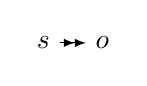
\begin{tikzpicture}[auto,>=latex, node distance=.75cm]
    \node[] (input) {$s$};
    \node[right of=input] (output) {$o$};
    \draw[->>] (input) -- (output);
\end{tikzpicture}
     &
     $\cong$
     &
\begin{tikzpicture}[auto,>=latex, node distance=.75cm]
    \node[] (input) {$s$};
    \node[block, right of=input] (D) {$\D$};
    \node[block, right of=D] (I) {$\I$};
    \node[right of=I] (output) {$o$};
    \draw[->>] (input) -- (D);
    \draw[->>] (D) -- (I);
    \draw[->>] (I) -- (output);
\end{tikzpicture}
\end{tabular}

\section{Incremental view maintenance}\label{sec:incremental}

The results in this section are not specific to databases, they hold
for any stream computations, but we hint about their applicability for
databases.

%Here we define IVM and analyze its properties.

%\begin{definition}
Given a stream operator $S: \stream{A} \to \stream{B}$ we define the
\defined{incremental version} of $S$ as:
%\begin{equation}\label{def:inc}
%\inc{Q} \defn \D \circ Q \circ \I.
%\end{equation}
%$\inc{Q}$ has the same ``type'' as $Q$: $\inc{Q}: \stream{A} \to \stream{B}$.

%The following diagram illustrates the intuition behind this
%definition:
\vspace{-2ex}
\begin{center}
\begin{tikzpicture}[auto,>=latex]
    \node[] (input) {$\Delta s$};
    \node[block, right of=input] (I) {$\I$};
    \node[block, right of=I] (Q) {$S$};
    \node[block, right of=Q] (D) {$\D$};
    \node[right of=D] (output) {$\Delta o$};
    \draw[->>] (input) -- (I);
    \draw[->>] (I) -- node (s) {$s$} (Q);
    \draw[->>] (Q) -- node (o) {$o$} (D);
    \draw[->>] (D) -- (output);
    \draw[decorate, decoration = {brace, raise=10pt}] (input) -- (output)
    node[pos=.5, above=13pt]{$\inc{S}$};
\end{tikzpicture}
\end{center}
\vspace{-1ex}
%\end{definition}

If $S$ computes on a stream $s$, then $\inc{S}$ computes on a stream
of changes to $s$.  If $S$ produces a stream $o$, then $\inc{S}$
produces the stream of changes to $o$.  Note that this definition does
not require $S$ to be a lifted function.

For an operator with multiple inputs and outputs we define the
incremental version by applying $\I$ to each input, and $\D$ to each
output, e.g.: $\inc{T}(a, b) \defn \D (T(\I(a), \I(b)))$.

%Notice that our definition of incremental computation is meaningful only for \emph{streaming}
%computations; this is in contrast to classic definitions, e.g.~\cite{gupta-idb95} which
%consider only one change.  Generalizing the definition to operate on streams gives us
%additional power, especially when operating with recursive queries.
%
%The following proposition is one of our central results:
$\inc{S}$ has many nice properties:

%\begin{proposition}(Properties of the incremental version):
%\label{prop-inc-properties}
%\begin{description}
%\item[inversion:] $Q\mapsto\inc{Q}$ is bijective; its inverse is $Q\mapsto \I\circ Q\circ\D$.
%\item[invariance:] $\inc{+} = +, \inc{(\zm)} = \zm, \inc{-} = -, \inc{\I}=\I, \inc{\D}=\D$
%\item[push/pull:] \label{prop-part-commutation}
%    $Q \circ \I = \I \circ \inc{Q}$; $\D\circ Q = \inc{Q}\circ\D$
%\item[chain:] $\inc{(Q_1\circ Q_2)} = \inc{Q_1}\circ\inc{Q_2}$ (Generalizes to multiple inputs.)
%\item[add:] $\inc{(Q_1 + Q_2)} = \inc{Q_1} + \inc{Q_2}$
%\item[cycle:] $\inc{(\lambda s. \fix{\alpha}{T(s,\zm(\alpha)}))} = \lambda s. \fix{\alpha}{\inc{T}(s,\zm(\alpha)})$
%\end{description}
%\end{proposition}
%
The \defined{chain rule} states that $\inc{(Q_1 \circ Q_2)} =
\inc{Q_1} \circ \inc{Q_2}$, i.e., these circuits are equivalent:

\noindent
\begin{tabular}{cr}
\begin{tikzpicture}[auto,>=latex]
  \node[] (input) {$\Delta i$};
  \node[block, right of=input] (I) {$\I$};
  \node[block, right of=I] (Q1) {$Q_1$};
  \node[block, right of=Q1] (Q2) {$Q_2$};
  \node[block, right of=Q2] (D) {$\D$};
  \node[right of=D] (output)  {$\Delta o$};
  \draw[->>] (input) -- (I);
  \draw[->>] (I) -- (Q1);
  \draw[->>] (Q1) -- (Q2);
  \draw[->>] (Q2) -- (D);
  \draw[->>] (D) -- (output);
\end{tikzpicture} &
$\cong$ \\
\begin{tikzpicture}[>=latex, node distance=.9cm]
  \node[] (input) {$\Delta i$};
  \node[block, right of=input] (I1) {$\I$};
  \node[block, right of=I1] (Q1) {$Q_1$};
  \node[block, right of=Q1] (D1) {$\D$};
  \node[block, right of=D1] (I2) {$\I$};
  \node[block, right of=I2] (Q2) {$Q_2$};
  \node[block, right of=Q2] (D2) {$\D$};
  \node[right of=D2] (output)  {$\Delta o$};
  \draw[->>] (input) -- (I1);
  \draw[->>] (I1) -- (Q1);
  \draw[->>] (Q1) -- (D1);
  \draw[->>] (D1) -- (I2);
  \draw[->>] (I2) -- (Q2);
  \draw[->>] (Q2) -- (D2);
  \draw[->>] (D2) -- (output);
\end{tikzpicture} &
$\cong$ \\
\begin{tikzpicture}[>=latex, node distance=1.2cm]
  \node[] (input) {$\Delta i$};
  \node[block, right of=input] (Q1) {$\inc{Q_1}$};
  \node[block, right of=Q1] (Q2) {$\inc{Q_2}$};
  \node[right of=Q2] (output)  {$\Delta o$};
  \draw[->>] (input) -- (Q1);
  \draw[->>] (Q1) -- (Q2);
  \draw[->>] (Q2) -- (output);
\end{tikzpicture}
\end{tabular}

\noindent In the database world, we can read this as: \textbf{to
  incrementalize a composite query you can incrementalize each
  sub-query independently}.  This gives us a simple deterministic
recipe reducing the incremental version of an arbitrary query to the
incremental version of its primitive operators.

The \defined{cycle rule} states that these circuits are equivalent:

\noindent
\begin{tabular}{m{4.4cm}m{.2cm}m{3cm}}
\begin{tikzpicture}[>=latex]
    \node[] (input) {$\Delta s$};
    \node[block, right of=input] (I) {$\I$};
    \node[block, right of=I] (f) {$T$};
    \node[block, right of=f, node distance=1.4cm] (D) {$\D$};
    \node[right of=D] (output) {$\Delta o$};
    \node[block, below of=f, node distance=.6cm] (z) {$\zm$};
    \draw[->>] (input) -- (I);
    \draw[->>] (I) -- (f);
    \draw[->>] (f) -- node (mid) {} (D);
    \draw[->>] (mid.center) |-  (z);
    \draw[->>] (z.west) -- ++(-.3,0) |- ([yshift=1mm]f.south west);
    \draw[->>] (D) -- (output);
\end{tikzpicture} & $\cong$ &
\begin{tikzpicture}[>=latex]
    \node[] (input) {$\Delta s$};
    \node[block, right of=input] (f) {$\inc{T}$};
    \node[right of=f, node distance=1.3cm] (output) {$\Delta o$};
    \node[block, below of=f, node distance=.6cm] (z) {$\zm$};
    \draw[->>] (input) -- (f);
    \draw[->>] (f) -- node (mid) {} (output);
    \draw[->>] (mid.center) |-  (z);
    \draw[->>] (z.west) -- ++(-.3,0) |- ([yshift=1mm]f.south west);
\end{tikzpicture}
\end{tabular}

\noindent
(We have omitted the labels on the inputs of $T$.) In other words, the
incremental version of a feedback loop around a query is just the
feedback loop with the incremental query for its body.  This result
will be useful for recursive queries.

%To execute incremental queries efficiently, we want to compute directly
%on streams of changes, without integrating them. The invariance property above shows
%that stream operators $+$, $-$, and $\zm$ are identical to their incremental versions.
%The following theorems generalize this to linear and bi-linear operators:

We call an operator $S$ \defined{linear} if it has the property that
$S(a+b) = S(a) + S(b)$ (where $+$ is the addition of streams).
%
%\begin{theorem}[Linear]\label{linear}
For a linear operator $S$ we have $\inc{S}=S$.
%\end{theorem}
%
This is very useful because many primitive database operations can be
implemented as linear operators: selection, projection, filtering,
grouping, parts of aggregation are all linear.  Moreover, the
following operators are linear: $-$, $z^{-1}$, $\I$, $\D$, $\lift{f}$
if $f$ is a linear function.

We call an operator $T$ with two inputs \defined{bilinear} if it
distributes over stream addition: $T(a+b, c) = T(a, c) + T(b, c)$, and
$T(a, c+d) = T(a, c) + T(a, d)$.  (Similar to multiplication's
distributivity over addition.)  In databases intersection, joins, and
Cartesian products are bilinear.

%\begin{theorem}[Bilinear]\label{bilinear}
Using infix notation, for a bilinear operator $\times$ we have:
\begin{eqnarray*}
\inc{(\Delta a \times \Delta b)} = \\
(\Delta a \times \Delta b ~+~ \zm(\I(\Delta a)) \times
\Delta b ~+~ \Delta a \times \zm(\I(\Delta b)) = \\
\Delta a \times \Delta b + \zm(a) \times \Delta b + \Delta a \times \zm(b)
\end{eqnarray*}

If we ignore the delay operators in this equation we recover the
well-known formula for join delta queries, e.g.,\cite{koch-pods10}.

%In pictures: \\
\noindent
\begin{tabular}{m{3.3cm}m{0cm}m{4cm}%m{0cm}m{2.8cm}
  }
\begin{tikzpicture}[auto,>=latex]
    \node[] (a) {$\Delta a$};
    \node[block, right of=a] (ai) {$\I$};
    \node[below of=a, node distance=.8cm] (midway) {};
    \node[below of=midway, node distance=.8cm] (b) {$\Delta b$};
    \node[block, right of=b] (bi) {$\I$};
    \node[block, right of=midway, node distance=1cm] (q) {$\times$};
    \node[block, right of=q] (D) {$\D$};
    \node[right of=D] (output) {$\Delta o$};
    \draw[->>] (a) -- (ai);
    \draw[->>] (b) -- (bi);
    \draw[->>] (ai) -- (q);
    \draw[->>] (bi) -- (q);
    \draw[->>] (q) -- (D);
    \draw[->>] (D) -- (output);
\end{tikzpicture} &
$\cong$ &
\begin{tikzpicture}[auto,>=latex]
  \node[] (input1) {$\Delta a$};
  \node[below of=input1, node distance=1.6cm] (input2) {$\Delta b$};
  \node[block, right of=input1, node distance=1cm] (I1) {$\I$};
  \node[block, below of=I1,node distance=.8cm] (ab) {$\times$};
  \node[block, right of=input2, node distance=1cm] (I2) {$\I$};
  \draw[->>] (input1) -- (I1);
  \draw[->>] (input2) -- (I2);
  \draw[->>] (input1) |- ([yshift=-1mm]ab.north west);
  \draw[->>] (input2) |- ([yshift=1mm]ab.south west);
  \node[block, right of=I1] (ZI1) {$\zm$};
  \node[block, right of=I2] (ZI2) {$\zm$};
  \draw[->>] (I1) -- (ZI1);
  \draw[->>] (I2) -- (ZI2);
  \node[block, right of=ZI1] (DI1) {$\times$};
  \node[block, right of=ZI2] (DI2) {$\times$};
  \draw[->>] (ZI1) -- (DI1);
  \draw[->>] (ZI2) -- (DI2);
  \node[block, circle, right of=ab, inner sep=0cm, node distance=2cm] (sum) {$+$};
  \draw[->>] (ab) -- (sum);
  \draw[->>] (DI1) -- (sum);
  \draw[->>] (DI2) -- (sum);
  \node[right of=sum, node distance=.8cm] (output) {$\Delta o$};
  \draw[->>] (sum) -- (output);
  \draw[->>] (input1) -- (DI2);
  \draw[->>] (input2) -- (DI1);
\end{tikzpicture}
%&
%$\cong$ &
%\begin{tikzpicture}[auto,>=latex,node distance=.7cm]
%  \node[] (input1) {$a$};
%  \node[below of=input1, node distance=1cm] (input2) {$b$};
%  \node[block, right of=input1, node distance=.5cm] (I1) {$\I$};
%  \node[block, right of=input2, node distance=.5cm] (I2) {$\I$};
%  \draw[->>] (input1) -- (I1);
%  \draw[->>] (input2) -- (I2);
%  \node[block, right of=I2] (ZI2) {$\zm$};
%  \draw[->>] (I2) -- (ZI2);
%  \node[block, right of=I1] (DI1) {$\times$};
%  \node[block, right of=ZI2] (DI2) {$\times$};
%  \draw[->>] (I1) -- (DI1);
%  \draw[->>] (ZI2) -- (DI2);
%  \node[block, circle, above of=DI2, inner sep=0cm, node distance=.5cm] (sum) {$+$};
%  \draw[->>] (DI1) -- (sum);
%  \draw[->>] (DI2) -- (sum);
%  \node[right of=sum, node distance=.5cm] (output) {$o$};
%  \draw[->>] (sum) -- (output);
%  \draw[->>] (input1) -- (DI2);
%  \draw[->>] (input2) -- (DI1);
%\end{tikzpicture}
\end{tabular}
%\end{theorem}

What is the intuition behind this diagram?  Let us consider the case
of Cartesian product $a \times b$.  The incremental product has inputs
$\Delta a = \D(a)$ and $\Delta b = \D(b)$.  What happens when we add a
row $x$ to relation $a$ (i.e., $\Delta a = x$)?  The new row $x$ will
appear in the output change combined with every row in the
\emph{previous version} of the \emph{full} relation $b$.  The operator
$\I(\Delta b)$ in fact computes relation $b$ from the stream $\Delta
b$ of changes, and $\zm$ applied to this value gives us its previous
version.  So the bottom $\times$ operator computes $x \times \zm(b) =
\Delta a \times \zm(\I(\Delta b))$, the change produced by the new row
$x$.  The top $\times$ operator performs the symmetric operation for
the changes of the $b$ relation.  The middle $\times$ operator
produces the results of changes to both inputs.

%Rewriting this statement using $\Delta a$ for the stream of changes to
%$a$ we get the familiar formula for incremental equi-joins:
%$\Delta(a\times b) =\Delta a \times \Delta b + a\times(\Delta b) +
%(\Delta a)\times b$; equi-joins are indeed bilinear.
%
